% Diese Vorlage soll einen Header bieten, der für die meisten Laborberichte und Hausaufgaben sinnvoll ist 
% und zudem einige nützliche Dinge in LaTeX erklären.
% Bisher ist sie von Steffen Brahtz und Thomas Lübbehüsen gepflegt worden, gerne können aber Sachen von anderen ergänzt werden.
\documentclass[
12pt,
a4paper,
bibliography=totoc,
listof=totoc,
headings=small,
parskip=half*, % Halbe Einzüge vor erste Zeile eines Absatzes, stattdessen Abstand zwischen Absätzen
]{scrartcl}

%%%%%%%%%%%%%%%%%%%%%%%%% Standardpakete %%%%%%%%%%%%%%%%%%%%%%%%%
\usepackage[utf8]{inputenc}        % Eingabe von Umlauten im Code
\usepackage[T1]{fontenc}           % Enkodierung von Output, böse Dinge passieren ohne dieses Package
\usepackage[ngerman]{babel}        % Deutsches Sprachpaket
\usepackage{scrhack}               % Warnungen bei KOMA-Skript fixen
\usepackage{amsmath}               % Mathematische Formeln
\usepackage{graphicx}              % Hinzufügen von Bildern / PDFs über \includegraphics{bildname}
\usepackage{caption}               % Erweiterte Captions für Bilder, Formeln, ...
\usepackage{physics}               % Zusätzliche wissenschaftliche Symbole und Differentialquotient mit \dd{...}
\usepackage[
headsepline,
footsepline,
automark
]{scrlayer-scrpage}                % Ändern von Kopf- & Fußzeile
\usepackage{hyperref}              % Links und Verweise in PDFs, hidelinks entfernt hässliche Rahmen um Links
\usepackage{siunitx}               % Wissenschaftlich korrektes Angeben von Zahlen / Einheiten (wichtig bei Hampe, Siaenen), u.A. Einheiten nicht kursiv
\usepackage[paper=a4paper,         % Seitenabstände und Papiergröße, hier recht geringe Einstellungen
left=25mm,                    
right=20mm,                   
top=15mm,                     
bottom=15mm,                  
includehead,includefoot            % Fuß- und Kopfzeile berücksichtigen
]{geometry}                   
                                
%%%%%%%%%%%%%%%%%%%%%%%%% Optionale Pakete, die aber praktisch sind %%%%%%%%%%%%%%%%%%%%%%%%%
%\usepackage{stix2}                 % Ändert die Schriftart! (und fügt Kugelintegral hinzu)
\usepackage{lastpage}              % Erlaubt "Seite 2 von x" im Footer, da es die Anzahl Seiten ausgibt
\usepackage{float}                 % Welches dann in Kombination mit [H] auch wirklich die Gleitumgebung mit dem Bild oder der Tabelle an die richtige Stelle packt, nämlich (H)ere 
\usepackage{array}                 % Matrizen in Latex
%\usepackage{esvect}                % Vektorpfeile mittels \vv{E}; ändert die Schriftart!
\usepackage{tabularx}              % Tabellen, die advanced sind
\usepackage{enumitem}              % Erweiterte Aufzählungen, bespielsweise alternative Aufzählungssymbole 
\usepackage{gensymb}               % Für Grad-Symbol \degree, Ohm: \ohm und einige mehr
\usepackage{textcomp}              % Zusätzliche Symbole wie \textdegree
\usepackage{icomma}                % Richtgen Abstand beim Dezimaltrennzeichen
\usepackage[all]{nowidow}          % Vermeidet "widows" (einzelne Zeilen auf nächster Seite die noch zum Absatz gehören)
\usepackage{chngcntr}              % Ändern von Nummerierung (Formeln, Bilder), z.B. Zählen innerhalb Kapitel
\usepackage[european,              % Europäischer Style für ciruitikz
straightvoltages,                  % Gerade Zählpfeile in DE
americaninductors,                 % Meist wird alte Norm mit Ami-Spulen genutzt
siunitx,                           % Integration von siunitx aktivieren
nooldvoltagedirection              % Neue Art für Spannungsrichtung auswählen, ist empfohlen
]{circuitikz}                      % circutikz: "Zeichnen" von Schaltungen im Code
\usepackage{subcaption}            % Bilder nebeneinander darstellen
\usepackage{csquotes}              % Für Zitate und um Warnung von babel zu unterdrücken
\usepackage[draft]{todonotes}      % \todo[inline]{beispiel}-Befehl, der Kommentare hinzufügt. Ausblenden der Todos durch ersetzen von "draft" durch "disable"
\usepackage{multirow}              % Für Tabellen: Mehrere Zeilen in einer Spalte miteinander verbinden
\usepackage{booktabs}              % Für das Excel2LaTeX-Addon, s.u. in Tipps
\usepackage{bigstrut}              % Für das Excel2LaTeX-Addon, s.u. in Tipps
\usepackage{cancel}                % Für durchgestrichenen Text (schlechte Messwerte zB) mit \cancel{text}
\usepackage{easyfig}               % Einfaches includen von Bildern z.B.: \Figure[caption={LOL}, width=\textwidth]{dateiname} (Labels sind automatisch \autoref{fig:dateiname})
\usepackage{listings}              % Includen von Code
\usepackage{xcolor}                % Eigene Farben definen
\usepackage{url}                   % Includenb von Links mit \url{http://thomas-harriehausen.de}

%%%%%%%%%%%%%%%%%%%%%%%%% Einstellung für Pakete und LaTeX %%%%%%%%%%%%%%%%%%%%%%%%%
% Bestimmte Warnung von chktex deaktivieren:
% chktex-file 46
% chktex-file 2
% chktex-file 1
% chktex-file 41

% Einstelllungen für das siuntix-Paket
\sisetup{
    per-mode=fraction,             % Einheiten als Brüche statt ^-1
    locale=DE,                     % Malpunkt, statt Kreuz
    output-decimal-marker={,},     % Komma als Dezimaltrennzeichen
    group-digits=true,             % Zifferngruppierung an/aus (in 3er Blöcken)
    group-separator=\text{~},      % Abstand als Trennzeichen für Zifferngruppierung
    group-minimum-digits=5,        % Ziffern ab minimal 5 Ziffern gesamt gruppieren
    detect-all,                    % Benutze gleiche Schriftarten wie im Text
    range-phrase=--,               % Komma in Range
    range-units=single             % Nur einmal die Einheit bei Range
}                                  
\DeclareSIUnit\divisor{div.}       % SIunitx: Volt pro Divisor, zB bei Schirmbildern      
\DeclareSIUnit\voltpeak{Vp}        % Für Vp in SI
\DeclareSIUnit\voltppeak{Vpp}      % Für Vpp in SI    

% Biblatex includen für Zitieren
\usepackage[style=numeric, 	       % Zitieren mit [1] statt [Ein05]
sorting=none,			           % Referenzen sotieren nach Ort des Auftauchen
backend=bibtex			           % Unterdrückt irgendeine Warnung
]{biblatex} 
%\addbibresource{../sources.bib}   % Optional, fügt sources.bib aus Oberverzeichnis hinzu
\addbibresource{sources.bib}       % Optional, fügt sources.bib aus gleichem Verzeichnis hinzu
\setcounter{biburllcpenalty}{7000} % für lange URLs im Quellverzeichnis
\setcounter{biburlucpenalty}{8000} %

% Für das todonotes package
\reversemarginpar                  % Randnotizen auf der linken Seite, da dort mehr Platz ist
\setlength{\marginparwidth}{2cm}   % Randnotizen-Breite festlegen, da das Paket sonst nicht funktioniert 

% Optional: Serifenlose Schriftart
%\renewcommand{\familydefault}{\sfdefault}

% Quellen ab x starten
%\newcommand{\quellenstart}{3} 
%\DeclareFieldFormat{labelnumber}{
%	\ifinteger{#1}
%	{\number\numexpr#1+\quellenstart\relax}
%	{#1}}

% Zählen innerhalb von Kapitel für Bilder / Gleichungen: <section>.<number>
\counterwithin{figure}{section}
\counterwithin{table}{section}
\counterwithin{equation}{section}

% Bilder in bestimmten Subfoldern müssen diesen Subfolder nicht im Dateinamen angeben
\graphicspath{{./fig/}{./bilder/}{./images/}{./figs/}}

% Titel alle etwas kleiner, Geschmackssache
%\usepackage[small]{titlesec}

% Höherer Zeilenabstand, Dirty Harrie will eigentlich 1.2, ist außerdem gut, weil's nach mehr Seiten aussieht
\linespread{1.15}

% Latex sorgt dafür, dass linebreaks stärker erzwungen werden und nicht Wörter über den Rand hinausragen; siehe https://texfaq.org/FAQ-overfull
\tolerance=7500
\pretolerance=200

% Etwas mehr Abstand zwischen den einzelnen aligns
\addtolength{\jot}{0.4em}

% Macht vertikalen Abstand in Tabellen größer, dieser ist default sehr klein
\renewcommand{\arraystretch}{1.15} 

% Kein Einschub bei Auflistungen, Geschmackssache
\setlist[enumerate]{leftmargin=*}

% Aufzählungen mit a) b) statt 1. 2.
\renewcommand{\labelenumi}{\alph{enumi}\)}

% Ersetzt alle * im Math-Environment durch richtige Malzeichen (cdot). Wenn * für konj. komplex oder ähnliches genutzt werden soll, dann auskommentieren
\mathcode`\*="8000
{\catcode`\*\active\gdef*{\cdot}}

% Indizes standardmäßig NICHT kursiv, da es nach DIN-Norm eher in Ausnahmen kursiv ist. Hilfreich für MET- und EMT-Labor
\makeatletter
\begingroup
\catcode`\_=\active
\protected\gdef_{\@ifnextchar|\subtextit\subtextup }
\endgroup
\def\subtextit|#1|{\sb{#1}}
\def\subtextup#1{\sb{\mathrm{#1}}}
\AtBeginDocument{\catcode`\_=12 \mathcode`\_=32768}
\makeatother

% Gleichung in Formel umbennen, Harrie mag das lieber
\renewcommand{\equationautorefname}{Formel}

\definecolor{mygreen}{RGB}{28,172,0} % color values Red, Green, Blue
\definecolor{mylilas}{RGB}{170,55,241}

\lstdefinelanguage{matlab}
{
    basicstyle=\ttfamily,
    breaklines=true,%
    keywords = {syms},
    morekeywords={matlab2tikz},
    keywordstyle=\color{blue},%
    morekeywords=[2]{1}, keywordstyle=[2]{\color{blue}},
    identifierstyle=\color{black},%
    stringstyle=\color{mylilas},
    commentstyle=\color{mygreen},%
    showstringspaces=false,%without this there will be a symbol in the places where there is a space
    numbers=left,%
    numberstyle={\tiny \color{black}},% size of the numbers
    numbersep=9pt, % this defines how far the numbers are from the text
    emph=[1]{for,end,break,imread,corr2},emphstyle=[1]\color{blue}, %some words to emphasise
}


%%%%%%%%%%%%%%%%%%%%%%%%% Eigene Befehle %%%%%%%%%%%%%%%%%%%%%%%%%
% Command hinzufügen, das einfach Linien für handschriftliche Notizen zeichnet. z.B. \lines{20} oder \lines[10pt]{20} (Abstand zwischen Zeilen, Anzahl Zeilen)
\usepackage{pgffor}
\newcommand{\lines}[2][8pt]{
    \foreach \n in {1,...,#2}{
        \rule{\textwidth}{0.5pt}\vspace{#1}\\
    }
}

%%%%%%%%%%%%%%%%%%%%%%%%% color %%%%%%%%%%%%%%%%%%%%%%%%%
\definecolor{listingbg}{cmyk}{0,0,0,0.05}
\definecolor{ostfalia-magenta}{cmyk}{0,1,0,0}
\definecolor{ostfalia-green}{cmyk}{0.3,0,1,0}
\definecolor{ostfalia-cyan}{cmyk}{0.78,0,0.32,0}
\definecolor{ostfalia-orange}{cmyk}{0,0.3,1,0}
\definecolor{ostfalia-yellow}{cmyk}{0,0.05,1,0}
\definecolor{ostfalia-violet}{cmyk}{0.86,0.96,0,0}
\definecolor{ostfalia-wf-blue}{cmyk}{1,0,0,0}
\definecolor{ostfalia-blue}{cmyk}{1,0.75,0,0.3}

% Kleines Underline, was sich gut für komplexe Zahlen eignet, z.B. \ul{U}_q
\newcommand{\ul}[1]{\underline{#1\mkern-1.5mu}\mkern 1.5mu}

% Text hervorheben als code / mono
\newcommand{\code}[1]{\ttfamily#1\rmfamily} % Beispiel: \code{AC}-Modus

% Normaler Text in Math-Environment mit Abstand vor und nach dem Text, nützlich um z.B. im align eine Formel zu beschreiben. z.B.: \desc{darin eingesetzt:}
\newcommand{\desc}[1]{{\hspace*{0,7 cm}\text{#1}\hspace*{0,7 cm}}}

% Buchstaben vor Subsections für Laborberichte (V2.2, A3.1, usw.) Benutzung mit \laborsubsection{V}{Überschriftstext}
\newcommand{\laborsubsection}[2] {
	\renewcommand{\thesubsection}{#1 \thesection.\arabic{subsection}}
	\subsection{#2}
	\renewcommand{\thesubsection}{\thesection.\arabic{subsection}}
}
% Einfacher Befehl, um Subsection wieder bei 1 starten, damit Wechsel von V 2.2 zu D 2.1 möglich ist
\newcommand{\resetlaborsectioncounter}{\setcounter{subsection}{0}}

% ABkürzungen mit korrekten Break
\newcommand*{\zb}{z.\,B.~\allowbreak}
\newcommand*{\ua}{u.\,a.~\allowbreak}

%%%%%%%%%%%%%%%%%%%%%%%%% Ausfüllen %%%%%%%%%%%%%%%%%%%%%%%%%
% Eigene Daten, werden dann in Header und PDF-Metadaten übernommen
\newcommand{\myAuthorA}{Max Mustermann, 70458112} 
\newcommand{\myAuthorB}{Max Musterfrau, 70458111}
\newcommand{\myGroup}{Gruppe X-24}
\newcommand{\myVersuch}{Versuch 1 - Spannungsteiler}
\newcommand{\myDate}{\today} % \today kann optional durch Text ersetzt werden
 
% Metadaten in PDF
\hypersetup{
    pdftitle={\myVersuch},
    pdfauthor={\myGroup: \myAuthorA{} \& \myAuthorB},
}

% Header und Footer setzen mit KOMA
\clearpairofpagestyles{}
\ihead{\myAuthorA \\ \myAuthorB}
\chead{\myGroup}
\ohead{\myVersuch}
%\automark{section}
\ifoot{\myDate}
\ofoot{Seite \thepage{} von \pageref{LastPage}}

%%%%%%%%%%%%%%%%%%%%%%%%% Tipps für TexStudio %%%%%%%%%%%%%%%%%%%%%%%%%
% Bessere Rechtschreibkorrektur in TexStudio hinzufügen: https://tex.stackexchange.com/a/282571/148289
% Tabellen-Autoformatierung mit dem blauen Button oben rechts in Tex-Studio
% Mehrere Zeilen gleichzeitig Bearbeiten mit gedrücktem STRG und Ziehen nach unten
% Word zu Latex Converter: https://www.docx2latex.com/ (Falls der Laborpartner zu inkompetent ist)
% Latex-Addin für Excel zum Exportieren von Tabellen, sehr empfehlenswert!: https://github.com/krlmlr/Excel2LaTeX/releases/latest (ZIP runterladen, extrahieren und einmal die xla-Datei ausführen)
% Excel-Addin zum (Batch-)Exportieren von Diagrammen als PNG: https://www.xltoolbox.net/de/
%%%%%%%%%%%%%%%%%%%%%%%%% ENDE des Headers %%%%%%%%%%%%%%%%%%%%%%%%%



\begin{document}
\section{Vollautomatische Messung des Ladevorganges}
\laborsubsection{V}{Entwurf der Messschaltung}
Wir haben uns für eine spannungsrichtige\todo{Hier fehlt noch Text} Messschaltung entschieden, da der $ 2,33 \cdot 9000 $ Widerstand der Spannungsmessung so hoch ist, dass er die Strommessung nur unwesentlich beeinflusst.


\section{Differenzier- und Integrierglied}
\laborsubsection{V}{Herleitung des Mittelwertes einer Rechteckimpulsfolge}
Die Spannung ist wie folgt definiert:
\begin{equation}
	u_p (t) =
	\begin{cases}
		U_{PH} ~ \text{für} ~ 0 \le t < t_{i} \\
		U_{PL} ~ \text{für} ~ t_{i} \le t < T
	\end{cases}
\end{equation}
Das Integral wird wie folgt gelöst:
\begin{align}
	\overline{u}_p & = \dfrac{1}{T} \cdot \Bigg [ \big [ U_{PH} \cdot t \big     ]_0^{t_{i}}   +    \big [  U_{PL} \cdot t \big ]_{t_{i}}^T    \Bigg ] \\
	\overline{u}_p & = \dfrac{1}{T} \cdot  \Bigg [ \Big ( U_{PH} \cdot t_{i} - 0 \Big ) + \Big ( U_{PL} \cdot T - U_{PL} \cdot t_{i} \Big ) \Bigg ]
\end{align}

Danach ergibt sich:
\begin{align}
	\overline{u}_p & = \dfrac{t_{i}}{T} \cdot (U_{PH}-U_{PL}) + U_{PL} \\
	               & = T_{v} \cdot (U_{PH}-U_{PL}) + U_{PL}
\end{align}


\section{Ladungspumpe und Spannungsvervielfacher}
\laborsubsection{V}{Herleitung einer Formel für Ausgangsspannung}
Die Kaskade kann in zwei Verdopplungsschaltungen nach \autocite[42]{moeller} aufgeteilt werden. Diese werden dann einzeln betrachtet.

$C_2$ würde mit $U_q$ über $C_1$ auf $2\cdot U_{q}$ aufgeladen werden, wenn die Durchlassspannungen der Dioden nicht vernachlässigt werden könnten. Berücksichtigt man diese aber, verringert sich diese Spannung um die Spannung, die an den beiden Dioden abfällt ($ 2 \cdot U_{F} $). Somit gilt für $U_{C_2}$:
\begin{equation}
	U_{C_2} = 2 \cdot U_{q} - 2 \cdot U_{F}
\end{equation}

$C_4$ in der zweiten Stufe wird nach dem gleichen Prinzip aufgeladen:
\begin{equation}
	\ul{U}_{C_4} = 2 \cdot U_{q} - 2 \cdot U_{F}
\end{equation}

\laborsubsection{V}{Entwurf der Messschaltung mit Oszilloskop}
Hier ist eine Referenz auf die \autoref{psch_diagramm}.
\begin{figure}[H]
	\centering
	\missingfigure{Hier muss noch ein Bild mit Spannungen hin}
	\captionof{figure}{Diagramm der Spannungen an Quelle und Kondensator}
	\label{psch_diagramm}
\end{figure}

\laborsubsection{V}{Vorbereitung zur Ladungspumpe}
\subsubsection{Vorlage Kaskadenschaltung}
\begin{figure}[H]
	\centering
	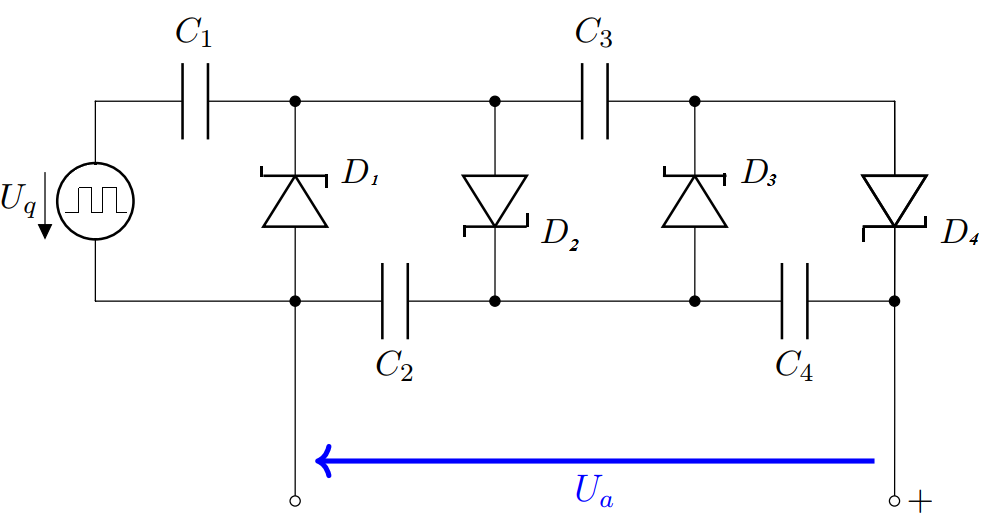
\includegraphics[width=0.8\textwidth]{schaltung}
	\captionof{figure}{4C/4D Kaskade als Vorlage zur Versuchsanordnung}
	\label{kaskadenschaltung}
\end{figure}

Und nochmal ein einfacher Include mit dem easyfig package. Referenz geht dann automatisch mit dem Dateinamen: \autoref{fig:schaltung}:
\Figure[caption={4C/4D Kaskade als Vorlage zur Versuchsanordnung}, width=0.8\textwidth,here]{schaltung}

Die Ausgangskapazität $C_A$ wird als Reihenschaltung der Kondensatoren $C_2$ und $C_4$ berechnet:
\begin{align}
	C_A = \dfrac{1}{\dfrac{1}{C_2}+\dfrac{1}{C_4}} = \dfrac{1}{\dfrac{1}{\SI{20}{\mu\farad}}+\dfrac{1}{\SI{20}{\mu\farad}}} = \SI{10}{\mu\farad}
\end{align}

Die zu erwartende Ausgangsspannung wurde berechnet:
\begin{equation}
	U_{C_2} =  U_{C_4}  = 2 \cdot U_{q} - 2 \cdot U_{F} = \SI{16}{\volt} - 2 \cdot \SI{300}{\milli\volt} = \SI{15,4}{\volt}
\end{equation}

Für $\dfrac{\dd{u_A}}{\dd{t}}$ gilt mit $I_A = \SI{10}{\milli\ampere}$:
\begin{equation}
	\dfrac{\dd{u_A}}{\dd{t}} = \dfrac{I_A}{C_A} = \dfrac{\SI{10}{\milli\ampere}}{\SI{10}{\mu\farad}} = \SI{1000}{\volt\per\second}
\end{equation}

\begin{table}[H]
	\centering
	\renewcommand{\arraystretch}{2} % Senkrechten Abstand für diese Tabelle erhöhen
	\setlength{\tabcolsep}{1.3em} % Horizontalen Abstand für diese Tabelle erhöhen
	\begin{tabular}{|c|c|c|c|c|c|}
		\hline
		$I_A$                  & $R_L $ & $U_A$ & $\dfrac{\dd{u_A}}{\dd{t}}$ (Messung) & $\dfrac{\dd{u_A}}{\dd{t}}$ (Rechnung) & $I_{umlade}$ \\ \hline
		\SI{1}{\milli\ampere}  &        &       &                                      & \SI{100}{\volt\per\second}            &              \\ \hline
		\SI{5}{\milli\ampere}  &        &       &                                      & \SI{500}{\volt\per\second}            &              \\ \hline
		\SI{10}{\milli\ampere} &        &       &                                      & \SI{1000}{\volt\per\second}           &              \\ \hline
	\end{tabular}
\end{table}

\resetlaborsectioncounter
\laborsubsection{D}{PSPICE-Simulation der Kaskade}
Die Schaltung wurde mit PSPICE simuliert, und mithilfe von Markern die Ausgangsspannung und der Umladestrom bestimmt. Um den Wechselanteil der Ausgangsspannung zu ermitteln, wurde vom angezeigten Wert der Durchschnittswert mittels \textit{AVG} abgezogen.

\begin{figure}[H]
    \centering
    \begin{subfigure}[b]{0.45\textwidth} % b steht für am Boden ausrichten, damit beide captions auf gleicher Höhe
        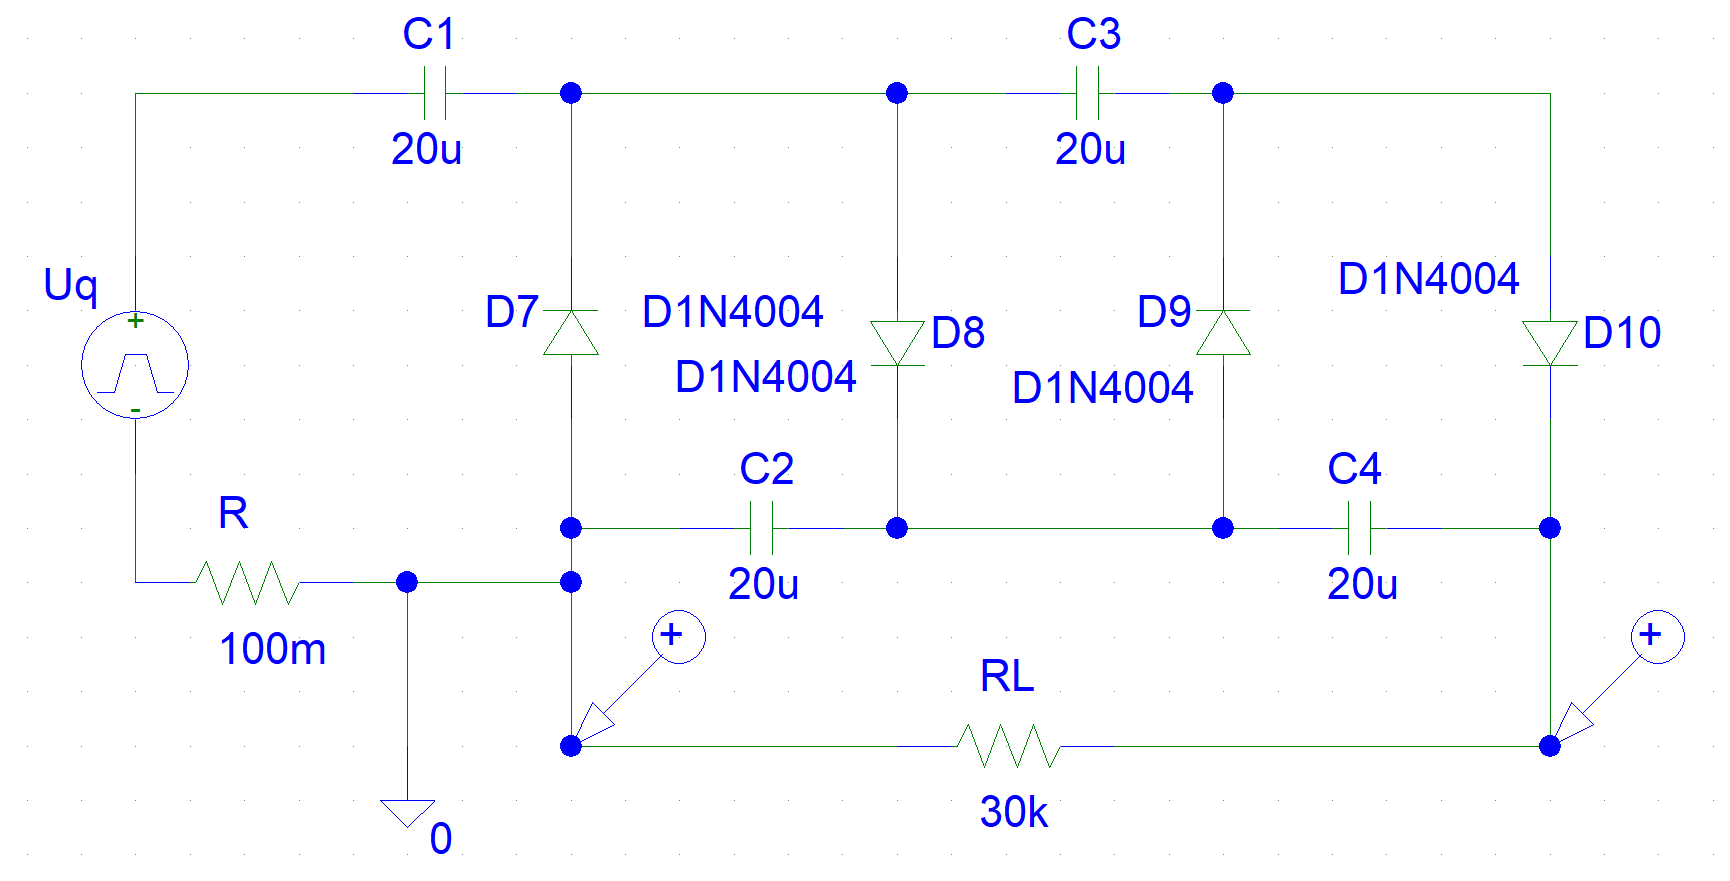
\includegraphics[width=\textwidth]{psch_kaskade}
        \subcaption{Simulation der Kaskadenschaltung (Marker für Spannungsmessung)}
        \label{psch_kaskade}
    \end{subfigure}
    \hfill % Um die beiden Figuren so weit wie möglich auseiannder zu machen
    % \hspace{0.1\textwidth} % Oder: Um einen festen Space zwischen den Figuren zu machen
    \begin{subfigure}[b]{0.45\textwidth}
    	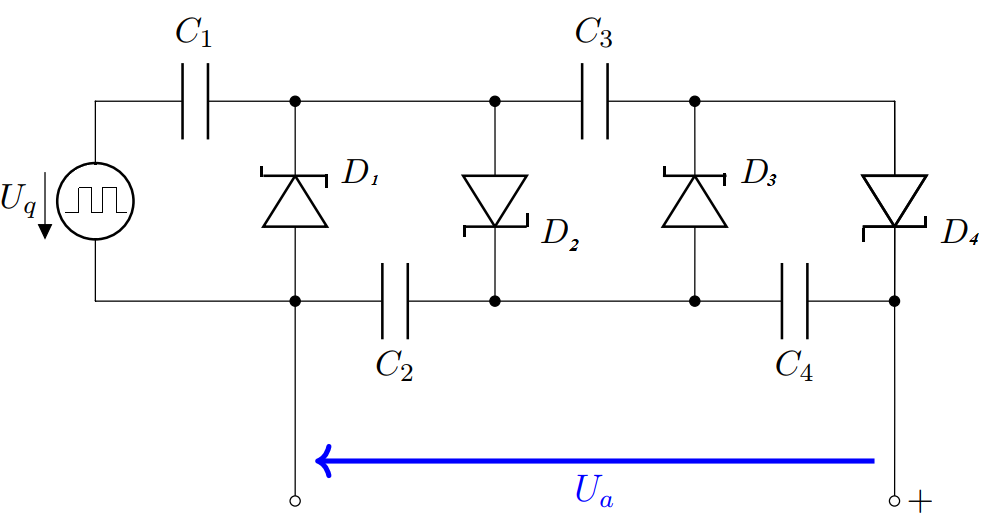
\includegraphics[width=\textwidth]{schaltung}
        \subcaption{4C/4D Kaskade als Vorlage zur Versuchsanordnung}
        \label{kaskadenschaltung_2}
    \end{subfigure}
    \caption{Gesamtdarstellung von irgendwas}
\end{figure}

\begin{lstlisting}[language=matlab]
syms x
c0 = 0;
c1 = 1;
c2 = 0.1;
c3 = -0.05;
X = 2; % X = 1;
Y1dach = c1*X + (3/4)*c3*X^3;
Y2dach = (1/2)*c2*X^2;
Y3dach = (1/4)*c3*X^3;
Y1eff = (1/sqrt(2)) * Y1dach;
Y2eff = (1/sqrt(2)) * Y2dach;
Y3eff = (1/sqrt(2)) * Y3dach;
Ygeseff = sqrt(Y1eff^2 + Y2eff^2 + Y3eff^2);

k2 = Y2eff/Ygeseff
k3 = Y3eff/Ygeseff
kges = sqrt(k2^2 + k3^2)

\end{lstlisting}


\printbibliography


\section*{Geräteliste}
\begin{table} [H]
	\begin{tabular}{|l|l|}
		\hline
		\textbf{Gerät }            & \textbf{Nummer }            \\ \hline
		Multimeter Keysight U1241C & AMES\_13, AMES\_14,AMES\_15 \\ \hline
		Stelltrafo                 & 27-15                       \\ \hline
		Stelltrafo                 & 29-24                       \\ \hline
		Ringkerntrafo              & 97-24                       \\ \hline
		Digitalmultimeter          & 40-24                       \\ \hline
	\end{tabular}
\end{table}

\end{document}